% This is samplepaper.tex, a sample chapter demonstrating the
% LLNCS macro package for Springer Computer Science proceedings;
% Version 2.20 of 2017/10/04
%
\documentclass[runningheads]{llncs}
%

\usepackage{graphicx}
\usepackage{algorithm}
\usepackage[noend]{algpseudocode}
\setcounter{secnumdepth}{2}
% \usepackage{amsmath}
% \usepackage{mathtools}
% Used for displaying a sample figure. If possible, figure files should
% be included in EPS format.
%
% If you use the hyperref package, please uncomment the following line
% to display URLs in blue roman font according to Springer's eBook style:
% \renewcommand\UrlFont{\color{blue}\rmfamily}

\begin{document}
%
%\title{STUD RRT*: Sampling-based Time-oriented Unrealistic planner using Doppler Effect Rapidly Exploring Random Tree Star}
\title{Deep Learning rooted Potential piloted RRT* for expeditious Path Planning}
%
%\titlerunning{Abbreviated paper title}
% If the paper title is too long for the running head, you can set
% an abbreviated paper title here
%
\author{
*YET TO BE PUBLISHED \inst{*} \\Snehal Reddy Koukuntla\inst{*}, Manjunath Bhat\inst{*}, Shamin Aggarwal \inst{*} and Rajat Kumar Jenamani}
%
% First names are abbreviated in the running head.
% If there are more than two authors, 'et al.' is used.
%
\institute{Indian Institute of Technology Kharagpur, India\\
\email{ksnehalreddy@iitkgp.ac.in, manjunathbhat9920@iitkgp.ac.in, shamin1998@iitkgp.ac.in,rajatkj11@gmail.com}}
%
\maketitle              % typeset the header of the contribution
%
\begin{abstract}
Randomised sampling based algorithms such as RRT and RRT* have a widespread use in path planning, but they tend to take considerable amount of time and space to converge towards the destination. RRT* with artificial potential field (RRT*-APF) is a novel solution to pilot the RRT* sampling towards the destination and away from the obstacles, thus leading to to faster convergence. But finding the potential function for each image is a gruelling task. In this paper we propose a machine learning based approach to tune the sensitive parameters of the RRT*-APF algorithm, which have a substantial effect on both rate of convergence and path length. 

\keywords{Path planning, Machine Learning, Robotics, RRT, Potential energy}
\end{abstract}
%
%
%
\section{\centering{Introduction}}
Current automated bots require the rapid motion of robots in a highly dynamic environment where agents try to excel in their task with superior planning and strategy. To achieve the above goals we need to design path planning algorithms that generate paths that are short in minimal amount of computational time and space. Traditional graph algorithms like Dijkstra and A* give the shortest path, but are very heavy in terms of computational load and hence cannot be used in the field of robotics which demands instantaneous results. On the other hand random sampling algorithms like Rapidly Exploring Random Trees (RRT) give stretched out paths and hence are not very feasible. RRT* solves this problem partially but brings the problem of slow rate of convergence towards the goal. 

Artificial Potential Field(APF) is an interesting and intuitive concept that solves the above problems, by biasing the random sampling towards the destination and away from the obstacles by inducing artificial fields. But traditional APF requires us to go over the wearying task of manually setting the extremely sensitive potential functions. Small changes in the potential functions can result in considerable change in both length of path generated and the rate of convergence and may also lead to the tree getting stuck in local minimum hence leading to infinite convergence time. 

The rest of the paper is organised as follows . Section 2  presents several extensions made to RRT .Section 3 formally explains our algorithm. Section 4 talks about the effectiveness of our algorithm in comparison to other path- planning algorithms. Section 5 briefs about the further modifications which can be done to our model to improve it.
\vspace{-2mm}  
\section{\centering{Background}}

\subsection{Rapidly-exploring Random Tree}
Here is a brief description of the method for a general configuration space, ${\cal C}$ (this can be considered as a general state space that might include position and velocity information). An RRT that is rooted at a configuration $q_{init}$ and has $K$ vertices is constructed using the following pseudo-code. 
Step 4 chooses a random configuration, $q_{rand}$, in ${\cal C}$. Alternatively, one could replace $rand\_conf$ with $rand\_free\_conf$, and sample configurations in ${\cal C}_{free}$ (by using a collision detection algorithm to reject samples in ${\cal C}_{obs}$).

It is assumed that a metric $\rho$ has been defined over ${\cal C}$. Step 5 selects the vertex, $q_{near}$, in the RRT, $G$, that is closest to $q_{rand}$

In Step 6 of $BUILD\_RRT$, $new\_conf$ selects a new configuration, $q_{new}$, by moving from $q_{near}$ an incremental distance, $\Delta q$, in the direction of $q_{rand}$. This assumes that motion in any direction is possible. If differential constraints exist, then inputs are applied to the corresponding control system, and new configurations are obtained by numerical integration. Finally, a new vertex, $q_{new}$ and a new edge is added from $q_{near}$ to $q_{new}$.


\begin{algorithm}
\caption{RRT algorithm}\label{RRT}
\begin{algorithmic}[1]
\Procedure{Build\_RRT}{$q_{init}$, $K$, $\Delta q$ }
\State $G.init(q_{init})$
\For{$ k = 1, 2, ..., K \do $}
\State $q_{rand}\gets rand\_conf();$
\State $q_{near}\gets nearest\_vertex(q_{rand}, G);$
\State $q_{new}\gets new\_conf(q_{near}, \Delta q);$
\State $G.add\_vertex(q_{new});$
\State $G.add\_edge(q_{near},q_{new});$
\EndFor
\State \textbf{return} $G$
\EndProcedure
\end{algorithmic}
\end{algorithm}

\begin{algorithm}
\caption{NEAREST\_VERTEX}\label{RRT}
\begin{algorithmic}[1]
\Procedure{nearest\_vertex}{$q, G$}
\State $d\gets \infty;$
\For{$v \in V \do$}
\If{$\rho(q,v) \leq d$}
\State $v_{new} = v;$
\State $d = \rho(q,v);$
\EndIf
\EndFor
\State \textbf{return} $v_{new}$
\EndProcedure
\end{algorithmic}
\end{algorithm}

\vspace{100mm}  
\subsection{RRT*}
-RRT*\cite{IJACSA} inherits all the properties of RRT and works similar to  RRT.  However,  it  introduced  two  promising  features called near  neighbor  search  and rewiring  tree operations.  Near  neighbor  operations finds  the  best  parent  node  for the new node before its insertion in tree. This process is performed within the area of a ball of radius defined by :

\vspace{3mm}

$k = \gamma (\frac{log(n)}{n})^{ \frac{1}{d} } $

\vspace{3mm}

\hspace{-6mm}where d is the search space dimension and γ is the planning constant    based    on    environment. Rewiring operation rebuilds the tree within this radius of area k to maintain the tree with minimal cost between tree connections. 

\begin{algorithm}
\caption{RRT*}\label{RRT*}
\begin{algorithmic}[1]
\Procedure{rrt\_star}{$T(v,e), Z_{init}$}
\State $T\gets InsertNode(\phi,Z_{init},T);$
\For{$i = 1, 2, ..., N \do $}
\State $Z_{rand}\gets Sample(i);$
\State $Z_{nearest}\gets Nearest(T,Z_{rand});$
\State $(Z_{nearest},U_{new} )\gets Steer(Z_{nearest},Z_{rand});$
\If{$Obstaclefree(Z_{new})$}
\State $Z_{near}\gets Near(T,Z_{new},V);$
\State $Z_{min}\gets Chooseparent(Z_{near},Z_{nearest},Z_{new});$
\State $T\gets InsertNode(Z_{min},Z_{new},T);$
\State $T\gets Rewire(T,Z_{near},Z_{min},Z_{new});$
\EndIf
\EndFor
\State\textbf{return} $T$
\EndProcedure
\end{algorithmic}
\end{algorithm}
  
\subsection{RT-RRT*}
RT-RRT*\cite{RT-RRT*} initializes the tree
with $x_a$ as its root. At each iteration, it expands and rewires the tree for a limited user-defined time (lines 5-6).  Then it plans a path from the current tree root for a limited user-defined amount of steps further . The planned path is a set of nodes starting from the tree root,($x_0$,$x_1$,...,$x_k$).  At each iteration it moves the agent for a limited time to keep it close to the tree root,$x_0$.  When path planning is done and the agent is at the tree root, it changes the tree root to the next immediate node after $x_0$ in the planned path,$x_1$.  Hence, the agent to moves on the planned path on the tree towards the goal.


% \section{RRT}
% Rapidly-exploring Random Trees (RRT) algorithm grows a tree rooted at the source node. Random points are sampled which are added to the tree until the goal is reached. It is a simple and fast algorithm but has certain limitations. It does not guarantee convergence
% to an optimal path solution. 

\vspace{-5mm}
\subsection{Potential piloted-RRT*}
Potential guided directional-RRT*(PDG-RRT*)\cite{potential}Potential Based Path Planning methods treat the environment as a potential field such that the goal point attracts and the obstacles
repulse the agent. These methods stem from the original Artificial
Potential Field (APF) introduced in \cite{potential}.  A lot of research has been done on this algorithm to improve its convergence rate.

\begin{algorithm}
\caption{Potential Guided Directional-RRT* algorithm}\label{alg:PG-RRT}
\begin{algorithmic}[1]
\Procedure{Potential Guided Directional-RRT*}{$x_{init}$}
\State $V\gets \{x_{init}\}$
\State $E\gets \phi$
\For{$ i = 1, 2, 3$ . . . $nodes_{max}$ \do }
\State $x_{rand}\gets SampleFree(i)$
\State $x_{prand}\gets GradientDescent(x_{rand})$
\State $x_{nearest}\gets Nearest(V, x_{prand})$
\State $x_{node}\gets Steer(x_{nearest}, x_{prand})$
\If{ObstacleFree($x_{nearest}$, $x_{node}$)}
\State $V\gets V \cup \{x_{node}\}$ 
\State $E\gets E \cup \{(x_{nearest}, x_{new})\}$
\EndIf
\EndFor
\State \textbf{return} $G = (V,E )$
\EndProcedure
\end{algorithmic}
\end{algorithm}
% \vspace{-10mm}
% \section{Problem statement and motivation}

\section{\centering{Algorithm}}
\vspace{-1mm}
The previous works describe various ways in which the RRTs have been modified to improve the optimality, speed and dynamism of path generation. The potential piloted RRT* promises more optimal paths,but is not feasible as it has sensitive parameters to be tuned, the change it which can lead to drastic changes in the resultant path and those parameters have different values on different parts on the field.

\begin{figure}
\begin{center}
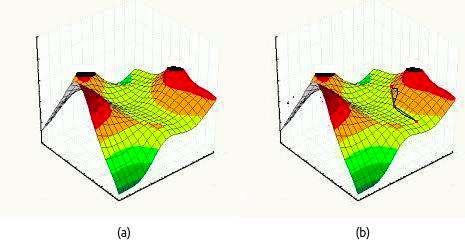
\includegraphics[scale=0.8]{images2_tog_new2.png}
    \caption{(a) The graph of superimposition of potential and frequency. (b) Straight line path is taken as cost in other planners marked in grey; actual path taken by our planner marked in black. The black patches mark infinity.} \label{fig1}
\end{center}
\end{figure}

\subsection{Potential field:}
Electrostatic field is a very  coarse-grained approximation of the potential field generated in the field. It is clearly evident that the destination should made to act like a positive charge and attract the tree to grow towards it. But since the obstacles should be avoided and hence they should be made to act like negative charges and repel the tree. At every point $x$ in the space, the potential is calculated for a particular charge as $\text{V_{i}}=\frac{\text{kQ_{i}}}{\text{r_{i}}}$ where $Q_{i}$ is the magnitude of the $i^{th}$ point charge (obstacle ), and $r_{i}$ is the distance of the point $x$ from it. The net potential at a point is given by :

\vspace{3mm}
$\sum_{i=1}^{n}V_{i}=k\sum_{i=1}^{n}\frac{\text{Q_{i}}}{\text{r_{i}}} + \text{k^\prime}\frac{\text{Q^\prime}}{\text{r^\prime}}$
\vspace{3mm}

\hspace{-5mm}Here $k$ and $k^\prime$ is a proportionality constant due to obstacles and destination respectively, and $n$ is the total number of charges. 

Now how much the tree should grow towards the destination relative to growing away from the obstacles, dependant on $k$ and $k^\prime$ is a very sensitive parameter and has serious implications(Fig 2 and Fig 3).
\vspace{3mm}

\begin{figure}
\begin{center}
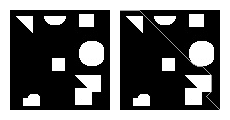
\includegraphics[scale=1.1]{merge_image(1).png}
    \caption{(a)The obstacle filled image. (b) The ideal path calculated using BFS and Dijkstra. (Section 3.2)} \label{fig1}
\end{center}
\end{figure}

\subsection{Ideal Potential Data Genration:}
To find the ideal constants of potential field , we first divided the field into 20X20 pixel sized grids whose centre is a good approximation for rest of the points in grid while finding the ideal potential functions at every point in the field. We found the ideal path by using BFS and Dijkstra from each of the grid's centre to the final destination. Using this ideal path we found the value of ideal k as follows -

\vspace{4mm}

Let the magnitude of net repulsive field be $k\sum_{i=1}^{n}\frac{\text{Q_{i}}}{\text{r_{i}}}$ and the magnitude of attractive field be $\frac{\text{Q^\prime}}{\text{r^\prime}}$

Let the angle between repulsive field vector and the ideal vector obtained from the ideal path be $\theta$ and let the angle between attractive field and the ideal vector be $\alpha$.

\vspace{4mm}

$k\sum_{i=1}^{n}\frac{\text{Q_{i}}}{\text{r_{i}}}{sin{\theta}}  =  \frac{\text{Q^\prime}}{\text{r^\prime}}{sin{\alpha}}$

\vspace{4mm}


From this expression k can be evaluated.

\vspace{4mm}

An example is shown in the figure below (Fig 3).
 \vspace{5mm}

\subsection{Training:}
The position of the obstacle is an important determinant of the RRT* Tree. So is the area of the obstacle. So we took the centres of the each obstacle blob and the total area of the obstacles as the features of the neural network. We designed the cost function by comparing the predicted path after an epoch and the ideal path by comparing the path coordinate lists using mean square error. With this custom error function we built a neural network with the help of Keras. We had two hidden layers. We used 5 fold cross validation to improve the neural network. We also made use Adam's optimizer. Using this we predicted the potential function. We then used the potential function thus predicted to run an RRT* APF tree and an example is shown in Fig. 3.
\vspace{10mm}
\begin{figure}
\begin{center}
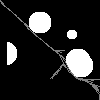
\includegraphics[scale=1.5]{img_bam.png}
    \caption{ The tree growth and piloted sampling of the nodes in RRT-Star with APF for the trained value of Potential Function. The tree converges directly to the destination and provides a very good approximation of the shortest path.} \label{fig1}
\end{center}
\end{figure}

\section{\centering{Results and Improvements:}}
\subsection{Time of convergence:}
The RRT* tree with the predicted values of potential functions converged faster than normal RRT* tree. For non ideal potential values, normal RRT* tree would get stuck at local minima which was being avoided by the predicted values.

The following table show the comparison between RRT* tree and the RRT* APF tree with predicted potential functions, wrt. to the time of covergence.

\vspace{10mm}
\begin{center}
\begin{tabular}{ |p{1cm}||p{3cm}|p{3cm}|  }
 \hline
 \multicolumn{3}{|c|}{Time of Convergence} \\
 \hline
 S.No. & RRT* &DL RRT* APF\\
 \hline
 1   & 3.58    &5.47\\
 2&   4.56  & 5.81   \\
 3 &4.28 & 6.31\\
 4    &5.96 & 6.42\\
 5&   3.42 & 5.92 \\

 \hline
\end{tabular}
\end{center}



\begin{figure}
\begin{center}
\includegraphics[scale=0.65]{stuckyy.png}
    \caption{ An illustration of a case where the tree gets stuck in a local minimum, due to highly unsuitable value of Potential Function, which is avoided using learning techniques}\label{fig1}
\end{center}
\end{figure}

\subsection{Width of the tree:}
The width of the tree also reduced significantly implying that the predicted values of potential functions were close to the ideal ones. The images below show the comparison between RRT* and DL RRT* APF with respect to the width of the tree.

\begin{figure}
\begin{center}
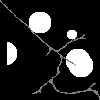
\includegraphics[scale=1.5]{tree.png}
    \caption{ The tree growth of RRT-Star with APF for a non-ideal value of Potential Function. It is evident that repulsion from the obstacle is not significant enough and that there is unnecessary branching of the tree. The final path is not a good approximation of the shortest path.(Fig 4)} \label{fig1}
\end{center}
\end{figure}
% \begin{figure}
% We conducted an experiment based on tree generation time given a set of obstacles. The experimental setup included ROS based communication nodes and a GUI based interactive platform for setting up the environment. This was performed on Linux 4.4.0-127-generic with 8 GiB memory and 2.3 GHz x 8 CPU.
% % \vspace{-1mm}
% \begin{table}[]
% \centering
% \caption{Comparison of time (in milli seconds) in generation of path}
% \label{Comparison with other planners}
% \begin{tabular}{@{}c|@{\hskip 0.1in}cccl@{}}
% \toprule
% \multirow{\textbf{Obstacles}} & \multicolumn{4}{c}{\textbf{Average Traversal Time}}              
% \\
%  & \textbf{PGD-RRT*} & \textbf{RRT*} & \textbf{RT-RRT*} & \textbf{Our planner} \\
%  \hline
% 5 & 4.1996  &  3.7078  &  3.7951  & 2.7958\\
% 7 & 4.2315  &  3.7912  &  3.8105  & 2.8110\\
% 9 & 4.2555  &  3.9105  &  3.8492  & 2.8862\\
% 10 & 4.2658 &  3.9824  &  3.8908  & 2.8873\\
% 12 & 4.3655 &  4.1473  &  4.1335  & 3.1080\\
% 15 & 4.4662 &  4.2194  &  4.3264  & 3.1866\\
% 18 & 4.6905 &  4.4505  &  4.5155  & 3.4242\\
% 20 & 4.9696 &  4.9191  &  4.9583  & 3.9823\\ 
% \end{tabular}
% \vspace{-6mm}
% \end{table}
% Thus, it can be seen that our planner takes nearly the same time to generate the tree given similar set of environmental conditions. Along with that, our planner provides a more optimised path. The average number of iterations required to find the path to each goal was 10.36 for our method and 18.43 for RT-RRT*.\\
% \vspace{-6mm}
% \subsubsection{Replanning}
% In a dynamic environment, the replanning of path is an important aspect. Moving obstacles when come along the path, a new path has to be found incorporating the new position of the obstacles. For better performance of agents, this replanning of path should take place in less amount of time. Our proposed path planner outperforms other planners in this, hence making it suitable for a real-time dynamic environment. With respect to the PGD-RRT*, our path planner is very quick in replanning as the tree growth does not take place again and again, but gets rewired when required. With respect to the RT-RRT*, our planner provides a more optimised path, which is clear from the illustration provided (fig 3) and Table 1. Our planner is based on a dynamic environment only and can be outperformed by other planners in a static environment.

% \begin{table}[]
% \centering
% \caption{Comparison of time (in milli seconds) in replanning of path}
% \label{Comparison of time in replanning of path}
% \begin{tabular}{@{}c|@{\hskip 0.1in}cccl@{}}
% \toprule
% \multirow{\textbf{Obstacles}} & \multicolumn{4}{c}{\textbf{Average Replanning Time}}              \\
%  & \textbf{PGD-RRT*} & \textbf{RRT*} & \textbf{RT-RRT*} & \textbf{Our planner} \\ 
% \hline
% 5 & 8.1996  &  8.7078  &  3.7958  & 3.7951\\  
% 7 & 8.2758  &  8.8213  &  3.8501  & 3.8491\\  
% 10 & 8.2783  &  8.8582  &  3.8614  & 3.8519\\  
% 11 & 8.2811  &  8.8607  &  3.8688  & 3.8564\\  
% 15 & 8.2902  &  8.9078  &  3.8891  & 3.8888\\  
% 18 & 8.3215  &  8.9303  &  3.9011  & 3.8997\\  
% 21 & 8.3414  &  8.9489  &  3.9114  & 3.9114\\  
% \end{tabular}
% \end{table}
% \\
% \vspace{-6mm}
% Our planner takes lesser tree generation time compared to the RT-RRT*, as it is biased in an intelligent way to reach the destination faster, using the concept of potential fields. Moreover, our planner features faster replanning as compared to PGD-RRT* as the tree growth does not take place again and again and is rewired. A similar advantage is seen over RRT* as well. The path generated is more optimised as compared to the RT-RRT* due to intelligent rewiring, which is evident from Table 1.
% \vspace{-2mm}
% \section{Conclusion}
% Our work focuses on a path planner with concepts from a variant of rapidly exploring random trees and artificial potential fields. They are merged innovatively, with concepts from various other domains, and a cost function redefined to suit a dynamic environment. This remains efficient in time with respect to tree growth and requires a lesser number of iterations for path generation, compared to that of similar planners.\\
% \vspace{-2mm}
% \subsection*{Future Work}
% In the future, we propose to research on how the acceleration of a robot can help in computing a more optimal path. Though the mathematics proposed in this paper can easily be extended to take acceleration into consideration, acceleration is not that easy to measure and a lot of noise comes in the way of the location data of the robots being received. Hence, our research aims to find an efficient solution to denoising the data post which we can take into consideration the acceleration, and if possible, other forms of kinetics.\\
% \\
\subsection*{Acknowledgement}
We sincerely thank Rajat Kumar Jenamani (rkj@iitkgp.ac.in), Ashish Kumar Gaurav (ashishkg0022@iitkgp.ac.in) for assisting us in this project and supporting us as and when required.
% \paragraph{Sample Heading (Fourth Level)}
% The contribution should contain no more than four levels of
% headings. Table~\ref{tab1} gives a summary of all heading levels.
% The 
% \begin{table}
% \caption{Table captions should be placed above the
% tables.}\label{tab1}
% \begin{tabular}{|l|l|l|}
% \hline
% Heading level &  Example & Font size and style\\
% \hline
% Title (centered) &  {\Large\bfseries Lecture Notes} & 14 point, bold\\
% 1st-level heading &  {\large\bfseries 1 Introduction} & 12 point, bold\\
% 2nd-level heading & {\bfseries 2.1 Printing Area} & 10 point, bold\\
% 3rd-level heading & {\bfseries Run-in Heading in Bold.} Text follows & 10 point, bold\\
% 4th-level heading & {\itshape Lowest Level Heading.} Text follows & 10 point, italic\\
% \hline
% \end{tabular}
% \end{table}


% \noindent Displayed equations are centered and set on a separate
% line.
% \begin{equation}
% x + y = z
% \end{equation}
% Please try to avoid rasterized images for line-art diagrams and
% schemas. Whenever possible, use vector graphics instead (see
% Fig.~\ref{fig1}).

% \begin{figure}
% \includegraphics[width=\textwidth]{fig1.eps}
% \caption{A figure caption is always placed below the illustration.
% Please note that short captions are centered, while long ones are
% justified by the macro package automatically.} \label{fig1}
% \end{figure}

% \begin{theorem}
% This is a sample theorem. The run-in heading is set in bold, while
% the following text appears in italics. Definitions, lemmas,
% propositions, and corollaries are styled the same way.
% \end{theorem}
%
% the environments 'definition', 'lemma', 'proposition', 'corollary',
% 'remark', and 'example' are defined in the LLNCS documentclass as well.
%
% \begin{proof}
% Proofs, examples, and remarks have the initial word in italics,
% while the following text appears in normal font.
% \end{proof}
% For citations of references, we prefer the use of square brackets
% and consecutive numbers. Citations using labels or the author/year
% convention are also acceptable. The following bibliography provides
% a sample reference list with entries for journal
% articles~\cite{ref_article1}, an LNCS chapter~\cite{ref_lncs1}, a
% book~\cite{ref_book1}, proceedings without editors~\cite{ref_proc1},

\begin{thebibliography}{99}
% \bibitem{ref_article1}
% Author, F.: Article title. Journal \textbf{2}(5), 99--110 (2016)

% \bibitem{ref_lncs1}
% Author, F., Author, S.: Title of a proceedings paper. In: Editor,
% F., Editor, S. (eds.) CONFERENCE 2016, LNCS, vol. 9999, pp. 1--13.
% Springer, Heidelberg (2016). \doi{10.10007/1234567890}

% \bibitem{ref_book1}
% Author, F., Author, S., Author, T.: Book title. 2nd edn. Publisher,
% Location (1999)

% \bibitem{ref_proc1}
% Author, A.-B.: Contribution title. In: 9th International Proceedings
% on Proceedings, pp. 1--2. Publisher, Location (2010)

% \bibitem{ref_url1}
% LNCS Homepage, \url{http://www.springer.com/lncs}. Last accessed 4
% Oct 2017
\bibitem{RT-RRT*}
Naderi, K., Rajamäki, J, Hämäläinen, P.:RT-RRT*: a real-time path planning algorithm based on RRT*. (2015)
\bibitem{tdp}
Bhushan, M., Agarwal, S., Gaurav, A.K., Nirala, M.K., Sinha, S., et al.: KgpKubs 2018 Team Description Paper. In: RoboCup 2018. (2018)
\bibitem{potential}
Khatib, O.:Real-Time Obstacle Avoidance for Manipulators and Mobile Robots (1986)
\bibitem{Springer}
Agarwal, S., Gaurav, A.K., Nirala, M.K., Sinha, S.:Potential and Sampling based RRT* for Real-Time Dynamic Motion Planning Accounting for Momentum in Cost Function. (2018)
\bibitem{MIT}
Brandon, D.L., Sertac, K., Jonathan, P.H.:Robust Sampling-based Motion Planning with Asymptotic Optimality Guarantees.
\bibitem{graphPlan}
Qureshi, A.H, Ayaz, Y.:Potential Functions based Sampling Heuristic For Optimal Path Planning. (2017)
\bibitem{IJACSA}
Noreem, I., Khan, A., Habib, Z.:Optimal Path Plainning using RRT* based Approaches: A Survey and Future Directions. (2016)
\bibitem{CS.RO}
Jonathan, D.G, Srinivasa, S.S., Barfoot, T.D.: Informed RRT*:Optimal Sampling-based Path Planning Focused via Direct Sampling of an Admissible Ellipsoidal Heuristic. (2014)
\bibitem{MIT}
Perez, A., Frazzoli, E., Walter ,M.R., et al.:Anytime Motion Planning using the RRT*. (2011)
\bibitem{SAGE journal}
Nasir, J., Fahad, I., et al.:RRT*-Smart:A Rapid Convergence Implementation of RRT*. (2013)

\end{thebibliography}
\end{document}
